Служба доставки <<Скедеф>> перевозит по воздуху посылки между несколькими городами. Какие-то из этих городов являются узлами и в них установлены специальные устройства для обработки посылок. Каждый из самолётов компании <<Скедеф>> летает туда и обратно между одной из пар городов, и перевозит посылки в любом из двух направлений, если это требуется.  

Чтобы перевезти посылку из одного города в другой, её необходимо провезти, используя последовательные перелёты через города, при этом на каждом перелёте посылка перевозится между парой городов, обслуживаемой одним из самолётов. Более того, в этой последовательности городов должен быть хотя бы один узел.

Для облегчения подборки маршрута, компания <<Скедеф>> хочет закодировать длины кратчайших последовательностей перелётов из каждого города в каждый узел и записать коды на метке каждой из посылок. Длина кратчайшей последовательности перелётов из узла в себя равна нулю. Очевидно, что требуется компактное представление этой информации.

Вам необходимо реализовать две процедуры --- \t{encode(N,H,P,A,B)} и \t{decode(N,H)}. Здесь $N$ --- количество городов, $H$ --- количество узлов. Города пронумерованы от $0$ до $N-1$, а узлами являются города с номерами от $0$ до $H-1$. Кроме того, $N \le 1000$ и $H \le 36$. $P$ --- количество пар городов, между которыми летает самолёт. Все пары городов различны как неупорядоченные пары. $A$ и $B$ --- это массивы размера $P$, и $(A[0], B[0])$ --- это первая пара городов, между которыми летает самолёт, $(A[1], B[1])$ --- вторая пара и т.д. 

Процедура \t{encode} должна построить такую последовательность битов, по которой
процедура \t{decode} сможет восстановить количество перелётов, необходимых для
перевозки посылки от каждого из городов до каждого из узлов. Процедура \t{encode} будет
передавать последовательность битов системе оценивания с помощью последовательных
вызовов процедуры \t{encode\_bit(b)}, где $b$ равно $0$ или $1$. Процедура \t{decode} будет получать последовательность битов от системы оценивания с помощью вызовов процедуры \t{decode\_bit}. При этом $i$-й вызов процедуры \t{decode\_bit} будет возвращать значение b, переданное $i$-му вызову \t{encode\_bit(b)}. Заметим, что вы должны удостовериться в том, что количество вызовов процедурой decode процедуры \t{decode\_bit} не будет 
превосходить количества сделанных процедурой encode вызовов процедуры \t{encode\_bit(b)}.

После декодирования информации о количестве необходимых перелётов, процедура
\t{decode} должна вызвать процедуру \t{hops(h,c,d)} для каждого из узлов $h$ и каждого из 
городов $c$ (в частности, и для узлов, и в случае $c=h$), сообщая минимальное количество
необходимых перелётов $d$, которые требуются для перевозки посылки между узлом $h$ и
городом $c$. Таким образом, вы должны сделать $N*H$ вызовов процедуры \t{hops(h,c,d)}.
Порядок этих вызовов не важен. Гарантируется, что всегда возможно перевезти посылку
между любым узлом и любым городом.

На оригинальном IOI было необходимо послать 2 отдельных файла с функциями \t{encode} и \t{decode}, но здесь они должны быть реализованы в одном файле. В любом случае, между вызовами \t{encode} и \t{decode} ваше решение будет перезапущено, по этому никаикие данные не могут быть сохранены. Они должны взаимодействовать толкьо с помощью вызовов функций  \t{encode\_bit}/\t{decode\_bit}. Но, для простоты тестирования, предоставленная вам версия грейдера вызовет обе функции в одном запуске. 


Реализуйте функции \t{encode} и \t{decode} в одном файле. Между их вызовами решение будет перезапущено, так что данные не сохранятся. Функции \t{encode} и \t{decode} должны взаимодействовать только через \t{encode\_bit} и \t{decode\_bit}

Для примера рассмотрим следующую схему:

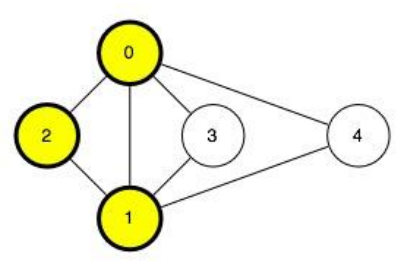
\includegraphics{SaveitSample.png}

На ней показаны пять городов $N=5$ связанных семью самолётами $P=7$. Города с номерами $0$, $1$ и $2$ являются узлами $H=3$. Для доставки посылки между узлом с номером $0$ и городом с номером $3$ необходим один перелёт, а для доставки посылки между узлом с номером $2$ и городом с номером $3$ необходимо два перелёта.

Значения $d$, которые процедура \t{decode} должна передать процедуре \t{hops(h,c,d)}, приведены в таблице ниже:

\begin{tabular}{|l|l|l|l|l|l|}
\hline
  & 0 & 1 & 2 & 3 & 4 \\ \hline
0 & 0 & 1 & 1 & 1 & 1 \\ \hline
1 & 1 & 0 & 1 & 1 & 1 \\ \hline
2 & 1 & 1 & 0 & 2 & 2 \\ \hline
\end{tabular}